\documentclass[a4paper,oneside,10pt]{report}
\usepackage{cite}
\usepackage[utf8]{inputenc}
\usepackage[francais]{babel}
\usepackage{enumerate}
\usepackage{fancyhdr}
\usepackage[nodisplayskipstretch]{setspace} 
\usepackage[dvips,a4paper]{geometry}
\usepackage{titlesec} 
\usepackage[hang,small,bf]{caption}
\usepackage{footmisc}
\usepackage{chngcntr}
\usepackage{moreverb}
\usepackage{color}
\usepackage{xcolor}
\usepackage{listings}
\usepackage{caption}
\usepackage{graphicx}
\usepackage{amsmath,amssymb,amsfonts}
\usepackage{colortbl,booktabs}
\usepackage{float}
\usepackage{pgfplots,pgfplotstable}
\usepackage{xspace}
\usepackage{tikz}
\usetikzlibrary{arrows,patterns,plotmarks,shapes,snakes,er,3d,automata,backgrounds,topaths,trees,petri,mindmap}
\usepackage[colorlinks=true,linkcolor=black,bookmarkstype=toc,linktocpage=true]{hyperref}
\counterwithout{footnote}{chapter}
\usepackage{amssymb,amsmath}

\setstretch{1.2}
%\setlength{\captionmargin}{0pt}
%\setlength{\headheight}{15pt} 
\geometry{lmargin=2.5cm,rmargin=2.5cm,vmargin=4cm}


\setlength{\parindent}{1cm}

%\renewcommand{\thechapter}{\Roman{chapter}}
\titleformat{\chapter}[display]
{\bfseries\Large}
{\filleft\MakeUppercase{\chaptertitlename} \Huge\thechapter}
{4ex}
{\titlerule
\vspace{2ex}%
\filright}
[\vspace{2ex}%
\titlerule]

\renewcommand*\thepart{\arabic{part}}%
\titlespacing*{\chapter}{0pt}{-60pt}{40pt}
\pagestyle{plain} 
\fancyhf{} 
\setlength{\footskip}{30pt} 
\setlength{\textheight}{646pt}
\setlength{\hoffset}{0pt}
\cfoot{\thepage} 
\renewcommand{\headrulewidth}{1.2pt}
\lhead{\leftmark}
\setlength{\skip\footins}{1cm}
\setlength{\footnotesep}{0.3cm}
\renewcommand{\footnotelayout}{\scriptsize}
\renewcommand{\chaptermark}[1]{\markboth{\footnotesize{#1}}{}}
\setstretch{1.2}
\pagenumbering{arabic}
\renewcommand\lstlistingname{Programme}
\renewcommand\lstlistlistingname{Programme}
\lstset{
		language=C++,
 basicstyle=\setstretch{1}\footnotesize\ttfamily,
 numbers=left,
 numberstyle=\scriptsize,
 numbersep=4pt,
 tabsize=2, 
 extendedchars=true,
 breaklines=true,
 keywordstyle=\color{red},
		 commentstyle=\color{gray},
 	 frame=b,
 stringstyle=\color{blue}\ttfamily,
 showspaces=false,
 showtabs=false,
 xleftmargin=17pt,
 framexleftmargin=17pt,
 framexrightmargin=5pt,
 framexbottommargin=4pt,
 showstringspaces=false,
		 }
\DeclareCaptionFont{white}{\color{white}}
\DeclareCaptionFormat{listing}{\colorbox[gray]{0.70}{\parbox{\textwidth}{\hspace
{15pt}#1#2#3}}}
\captionsetup[lstlisting]{format=listing,labelfont=white,textfont=white,
singlelinecheck=false,margin=0pt,font={bf,footnotesize}}
\setlength{\parindent}{0cm}

\newcommand{\W}{\mathbf{W}}
\newcommand{\w}{\mathbf{w}}



\begin{document}
\def\chaptername{travaux pratiques} 
\pagestyle{plain}
\setstretch{1.2}

\chapter{Déformation d'une membrane}

On propose ici, d'étudier un exemple de problème physique et de le résoudre via la librairie éléments finis \texttt{Feel++}.
\section{Implement in \texttt{Feel++} this model, visualise the results for some parameters in scaled coordinates (i.e in $\xi$)}

\subsubsection{1. Initialize $T$, $A$, $R$, $x_0$, $y_0$, and $\sigma$}

On initialise les constantes via un fichier \texttt{membrane.cfg}, cela évite de devoir recompiler pour modifier les paramètres. Le passage à l'exécution se fait via l'appel  \texttt{./my\_program --config-file=membrane.cfg}

\begin{center}
\begin{minipage}{\textwidth}
\begin{lstlisting}[label=code2,caption=Contenu du fichier membrane.cfg ]
T = 10.0 #Tension
A = 1.0 #Pressure Amplitude
R = 0.3 #Radius
x0 = 0.2 #Localization x0 of pressure amplitude
y0 = 0.4 #Localization y0 of pressure amplitude
sigma = 10 # Width of Gaussian
\end{lstlisting}
\end{minipage}
\end{center}

Dans le fichier source on définit ces paramètres comme passés en option,


\begin{center}
\begin{minipage}{\textwidth}
\begin{lstlisting}[label=code2,caption=membrane.cpp - Définition des options]
  po::options_description options ( "Membrane options ") ;
  options.add_options()
  ( "T", po::value<double>()->default_value(1.0), "Tension" )
  ( "x0", po::value<double>()->default_value(0.0), "x-coordinate" )
  ( "y0", po::value<double>()->default_value(0.0), "y-coordinate" )
  ( "sigma", po::value<double>()->default_value(0.02), "sigma" )
  ( "R", po::value<double>()->default_value(0.3), "Radius" )
  ( "A", po::value<double>()->default_value(1.0), "Amplitude" );
\end{lstlisting}
\end{minipage}
\end{center}


Bien évidemment, une fois ces paramètres lus dans le fichier \texttt{cfg}, il faudra les stocker (opération de casting) sous forme de doubles manipulables par le programme. Cela se fait via le bloc suivant,

\begin{center}
\begin{minipage}{\textwidth}
\begin{lstlisting}[label=code2,caption=membrane.cpp - cast des options]
  double T = option(_name="T").as<double>();
  double x0 = option(_name="x0").as<double>(); 
  double y0  = option(_name="y0").as<double>();
  double sigma = option(_name="sigma").as<double>();
  double R = option(_name="R").as<double>();
  double theta = option(_name="theta").as<double>();
  double A = option(_name="A").as<double>();
\end{lstlisting}
\end{minipage}
\end{center}

\subsubsection{2. Create a mesh over the unit circle}

Le cercle unité est créé via l'appel, \texttt{auto mesh = unitCircle();}:  ici on considèrera une approximation géométrique d'odre 1.

\subsubsection{3. Make an expression object for the scaled pressure function $f$}

Grace à \texttt{ginac} (librairie de calcul formel) on peut définir un object de type expression associé à notre fonction $f$. \texttt{Ginac} se chargera de la traduction pour l'évaluation numérique ultérieure. La déclaration est la suivante,
\begin{center}
\begin{minipage}{\textwidth}
\begin{lstlisting}[label=code2,caption=membrane.cpp - fonction f via Ginac expression]
auto f=expr("4*exp(-0.5*(pow((R*x-x0)/sigma,2)) - 0.5*(pow((R*y-y0)/sigma,2))):x:y:R:sigma:x0:y0"); 
//Solution exacte (via ginac)
auto we = expr("1-x*x-y*y:x:y");
\end{lstlisting}
\end{minipage}
\end{center}

Note : les paramètres passés après les ":" sont les variables/constantes numériques de la fonction.


\subsubsection{3. Define the $a$ (bilinear) and $L$ (linear) formulas in the variational problem for $\xi$ and compute the solution}

Le problème est celui d'un Laplacien 2D avec condition de Dirichlet homogène sur le bord $\xi = 0 \mbox{ sur } \partial \Omega$. On définit une approximation par des élements $\mathbb{P}2$ de Lagranges, ensuite on définit les formes linéaire et bilinéaire. La condiition au bord est imposée par le mot clé \texttt{on},

\begin{center}
\begin{minipage}{\textwidth}
\begin{lstlisting}[label=code2,caption=membrane.cpp - Espace et forme linéaire/bilinéaire]
  auto Xh = Pch<2>(mesh);
  //Trial function : Solution
  auto w = Xh->element();
  //Test function
  auto v = Xh->element();
  //Deflection
  auto d = Xh->element();
  //Linear form
  auto l = form1(_test=Xh);
  l= integrate(_range=elements(mesh),
               _expr= f*id(v) );
  //Bilinear form
  auto a = form2(_test=Xh,_trial=Xh);
  a = integrate( _range=elements(mesh),
                 _expr=gradt(w)*trans(grad(v)) );
  //Homogene Dirichlet boundary condition
  a+=on(_range=boundaryfaces(mesh), _rhs=l, _element=w, _expr=cst(0.));
\end{lstlisting}
\end{minipage}
\end{center}



\subsubsection{4. Plot the mesh, $\xi$, and $f$}
Afin de tracer le maillage, $\xi$ et $f$, on exporte les resultats via l'\texttt{exporter} de \texttt{feel++}. Il faut bien évidemment projeter la fonction $f$sur les éléments du maillage afin de la visualiser plus tard.

\begin{center}
\begin{minipage}{\textwidth}
\begin{lstlisting}[label=code2,caption=membrane.cpp - export des résultats]
auto e = exporter( _mesh=mesh ); 
  //Solution
  e->add( "w", w );
  //Fonction f projete sur les elements du maillage
  e->add("f",vf::project(_space=Xh, _range=elements(mesh), _expr=f));
  e->save();
\end{lstlisting}
\end{minipage}
\end{center}

Rappel : ici $f$ représente la force de pression et $w$ la réponse de la membrane.
Ci-dessous les graphes générés avec \texttt{paraview} pour $\sigma = 1000$ et $\sigma = 0.01$ . On utilise ici le filtre \texttt{wrap by scalar} suivant la normale avec un coefficient égal à 1. Cela nous permet une visualisation 3D du problème.

\begin{figure}[!h]
\begin{center}	
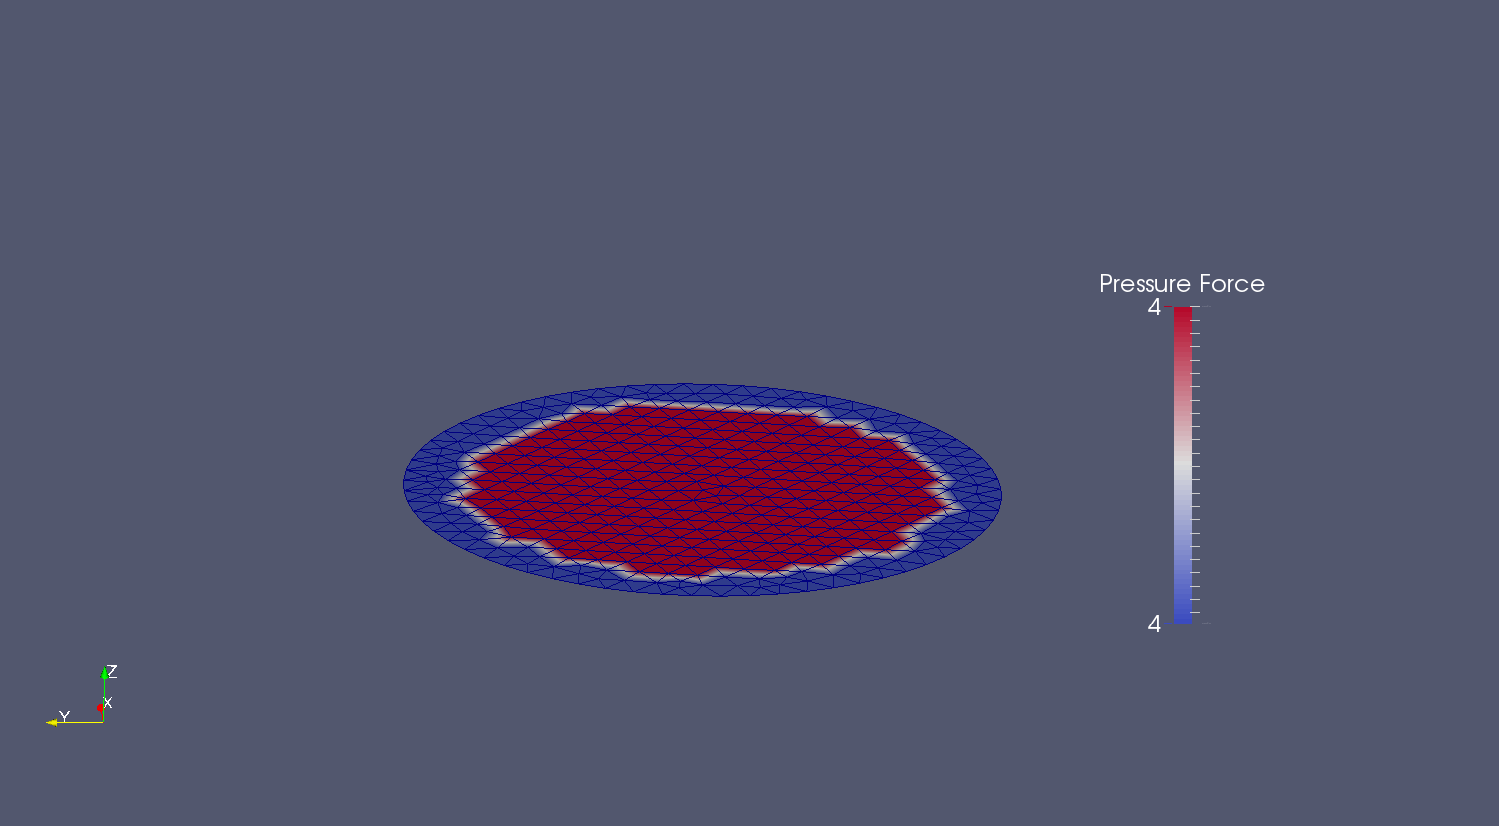
\includegraphics[width=\textwidth]{pressure_sig1000.png}
\caption{\label{fig1}Force de pression $f$ pour $\sigma = 1000$} 
\end{center}
\end{figure}

\begin{figure}[!h]
\begin{center}	
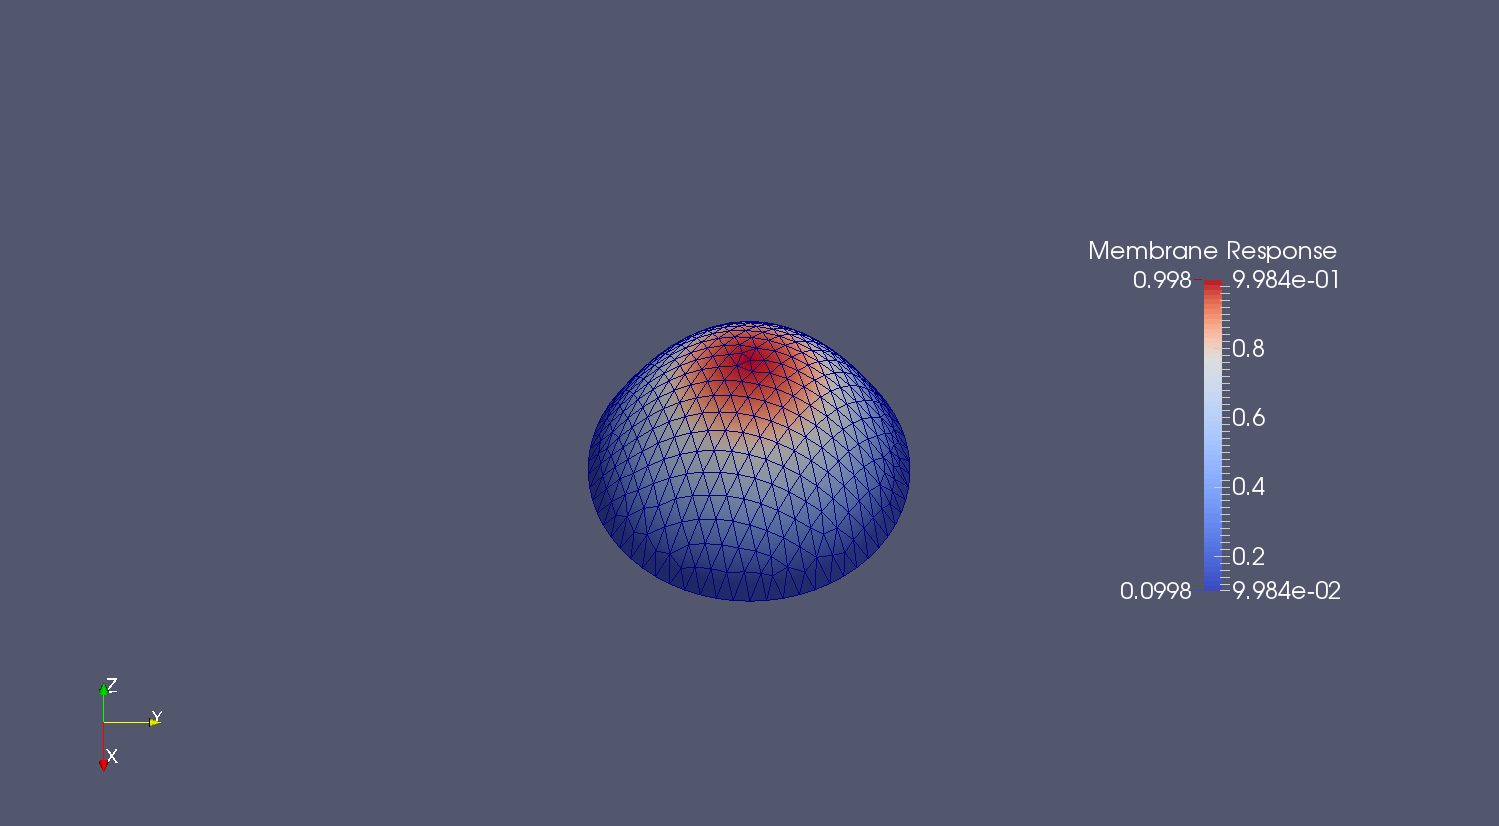
\includegraphics[width=\textwidth]{w_sig1000.png}
\caption{\label{fig1}Réponse de la membrane $w$ pour $\sigma = 1000$} 
\end{center}
\end{figure}

\begin{figure}[!h]
\begin{center}	
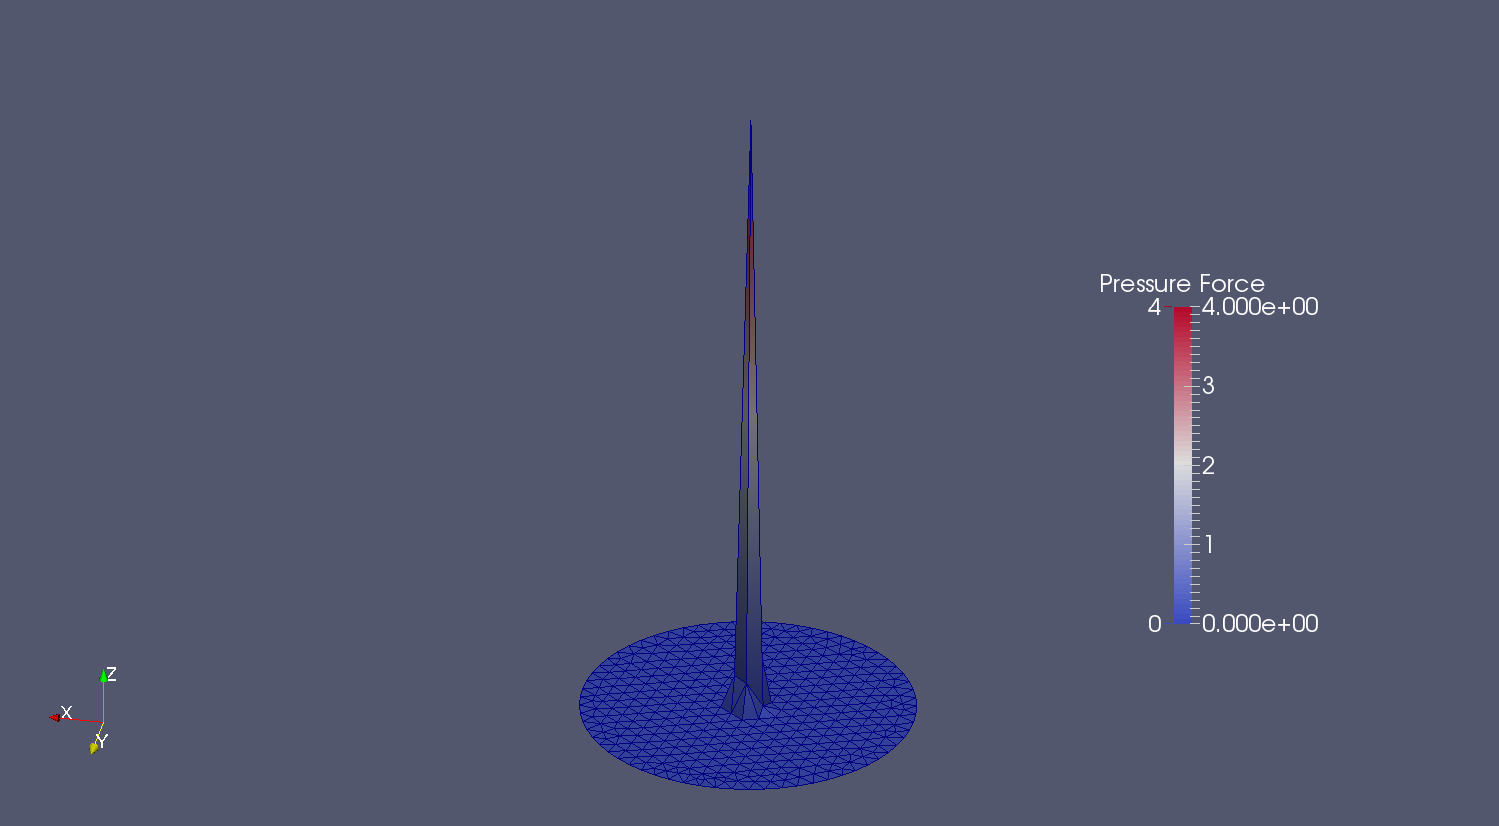
\includegraphics[width=\textwidth]{pressure_sig001.png}
\caption{\label{fig1}Force de pression $f$ pour $\sigma = 0.01$} 
\end{center}
\end{figure}

\begin{figure}[!h]
\begin{center}	
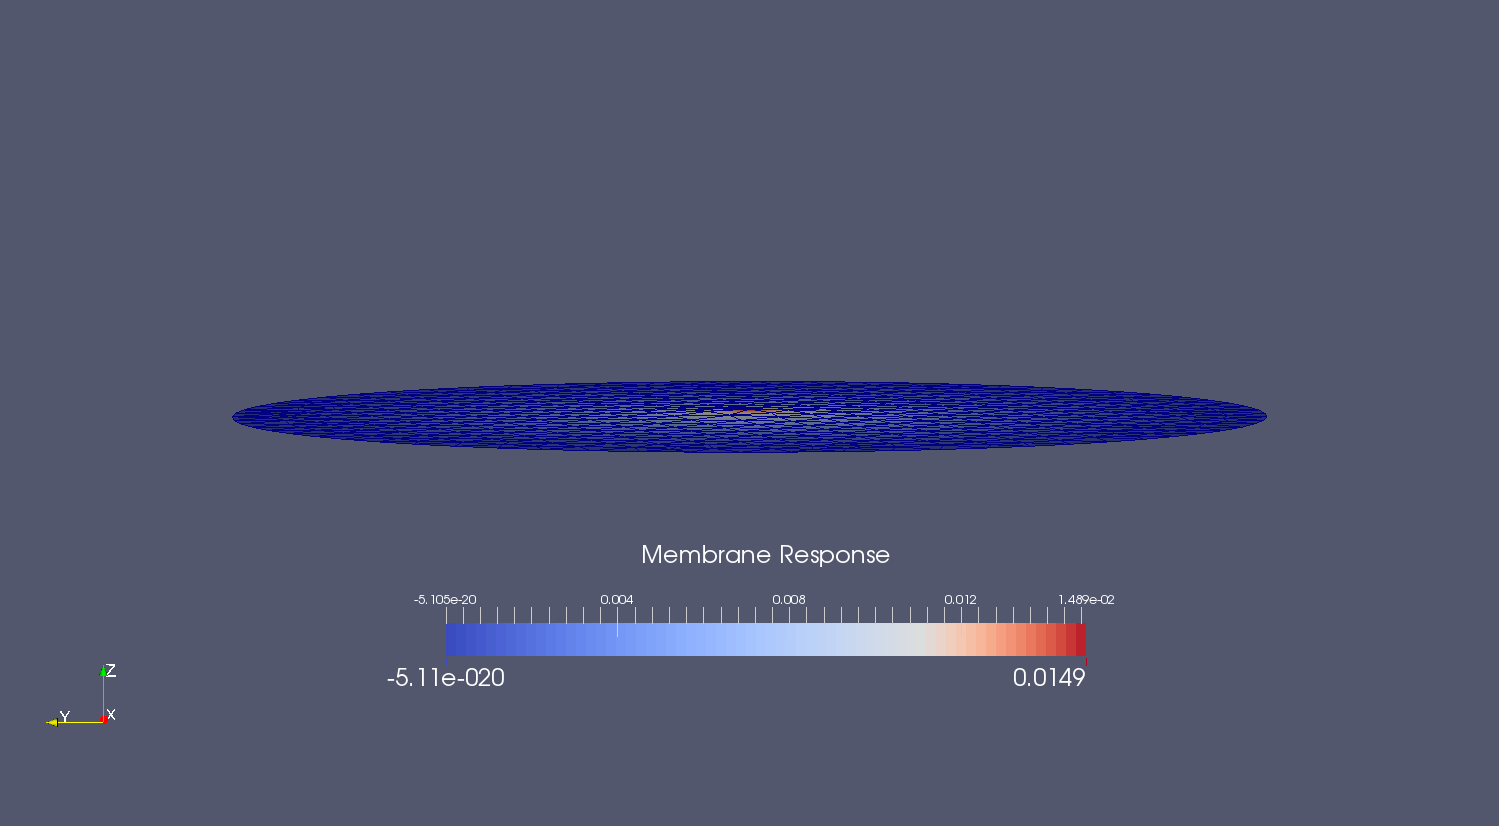
\includegraphics[width=\textwidth]{w_sig001.png}
\caption{\label{fig1}Réponse de la membrane $w$ pour $\sigma = 0.01$} 
\end{center}
\end{figure}

On remarque bien que pour $\sigma$ très grand la force de pression $f$ est une fonction constante égale à 4 $\forall\ (x,y) \in \Omega$. Le second cas, $\sigma = 0.01$ est très intéressant car il montre l'effet régularisant/moyennant de l'opérateur Laplacien. En effet la force de pression appliquée est très "piquée" en un point alors que la membrane, elle, se déforme de manière très régulière.

\subsubsection{5. Write out the maximum real defections $\xi$ and $d$, this can be obtained using the \texttt{max} member function that
returns the maximum of the coefcients of an element of a function space.}

Afin de calculer ces quantités, on définit tout d'abord $d$, ensuite on utilise la sortie standard pour afficher les résultats. Ici on emploie l'appel à la fonction \texttt{normLinf} qui calcule le maximum atteint (en valeur absolue) sur tout le domaine $\Omega$.

\begin{center}
\begin{minipage}{\textwidth}
\begin{lstlisting}[label=code2,caption=membrane.cpp - definition de d]
  auto d = Xh->element();
  d=(A*R*R)/(8*pi*sigma*T)*u;

  std::cout << "max(d) = "
                << normLinf( _range=elements(mesh), _expr=idv(d), _pset=_Q<5>() )
                << "\n";
                
  std::cout << "max(w) = "
            << normLinf( _range=elements(mesh), _expr=idv(w), _pset=_Q<5>() )
            << "\n";  
      
\end{lstlisting}
\end{minipage}
\end{center}

Pour le jeu de paramètres $T=10.0$, $A = 1.0$, $R = 0.3$, $\theta = 0.2$ $x_0 = 0.5*R*\cos(\theta)$, $y_0 = 0.5*R*\sin(\theta)$ et $\sigma $= 0.01, on obtient
$\max(d) = 0.000519394$ au point $(-0.00209859,-0.0119205)$ et $\max(\xi) = 0.000519394$ au point $(-0.00209859,-0.0119205)$.

\subsubsection{6. Verify numerically that at the limit $\sigma \rightarrow \infty$, in scaled coordinates we have that $w_e = 1 - x^2 - y^2$ on the unit disk. Check that for example $L^2$ of the error in $0$ for a $\sigma$ large enough. What typical value $\sigma$ should be enough to verify this result ?}
Afin de vérifier, la convergence en $0$ on définit tout d'abord via \texttt{Ginac} l'expression de la solution exacte $w_e$. Ensuite on calcule la différence en \texttt{normL2} entre la solution approchée $w$ et la solution exacte $w_e$ pour une valeur de sigma donnée. L'affichage se fait sur la sortie standard.
\begin{center}
\begin{minipage}{\textwidth}
\begin{lstlisting}[label=code2,caption=membrane.cpp - Calcul de la différence en norme L2]
  //Solution exacte
  auto we = expr("1-x*x-y*y:x:y");
  // Affichage sur la sortie standard
  std::cout << "|w-we|= "
            << normL2(_range=elements(mesh),
                      _expr=(idv(w)-we) )
            << "\n";
 \end{lstlisting}
\end{minipage}
\end{center}
On remarque que pour des paramètres $T=10.0$, $A = 1.0$, $R = 0.3$, $\theta = 0.2$ $x_0 = 0.5*R*\cos(\theta)$, $y_0 = 0.5*R*\sin(\theta)$on obtient ,
\begin{center}
\begin{tabular}{|c|c|}
  \hline
  $\sigma$ &  $||w-w_e||_{L^2[\Omega]}$ \\
  \hline
  0.01 &  1.01824  \\
  0.1 & 0.64908 \\
  1.0 & 0.0170525 \\
  10 &  0.00305419\\
  50 & 0.0029544\\
  100 & 0.0029226\\
  1000 & 0.00292129\\
   \hline
\end{tabular}
\end{center}
On observe une convergence vers la valeur de $0.0029$ lorsque $\sigma \rightarrow \infty$. En effet, lorsque $\sigma$ (épaisseur de la gaussienne) est grand, la force appliquée à la membrane est extrêmement étalée en surface. De plus, analytiquement on constate lorsque $\sigma \rightarrow \infty$ on a $f \rightarrow  4$. De la même manière en injectant la solution $w_e$ on a $\Delta w_e = -4$ sur $\Omega$. Cet aspect a été vérifié numériquement en sous-section 4.  Ainsi une valeur de $\sigma\approx 50$ représente un étalement quasi-uniforme sur l'ensemble du domaine $\Omega$ (cercle unité).
\subsubsection{7. Complete source code of \texttt{membrane.cpp}}
\begin{center}
\begin{minipage}{\textwidth}
\begin{lstlisting}[label=code2,caption=membrane.cpp]
#include <feel/feel.hpp>
int main( int argc, char** argv ) {
  using namespace Feel;
  po::options_description options ( "Membrane options ") ;
  options.add_options()
  ( "T", po::value<double>()->default_value(1.0), "Tension" )
  ( "theta", po::value<double>()->default_value(0.2), "theta" )
   ( "sigma", po::value<double>()->default_value(0.02), "sigma" )
  ( "R", po::value<double>()->default_value(0.3), "Radius" )
  ( "A", po::value<double>()->default_value(1.0), "Amplitude" );
   Environment env( _argc=argc, _argv=argv,
                              _desc=options,
                              _about=about(_name="membrane",
                              _author="Feel++ Consortium",
                              _email="feelpp-devel@feelpp.org"));
                            
  double T = option(_name="T").as<double>();
  double theta = option(_name="theta").as<double>(); 
  double sigma = option(_name="sigma").as<double>();
  double R = option(_name="R").as<double>();
  double A = option(_name="A").as<double>();
  double x0 = 0.5*R*cos(theta);
  double y0 = 0.5*R*sin(theta);
  auto mesh = unitCircle();
  auto Xh = Pch<2>(mesh);
  auto w = Xh->element();
  auto v = Xh->element();
  auto d = Xh->element();
  auto we = expr("1-x*x-y*y:x:y");
  auto f=expr("4*exp(-0.5*(pow((R*x-x0)/sigma,2)) - 0.5*(pow((R*y-y0)/sigma,2))):x:y:R:sigma:x0:y0"); 
  //linear and bilinear form
  auto l = form1(_test=Xh);
  l = integrate(_range=elements(mesh),
                     _expr= f*id(v) );
  auto a = form2(_test=Xh,_trial=Xh);
  a = integrate(_range=elements(mesh),
                      _expr=gradt(w)*trans(grad(v)) );
  a+=on(_range=boundaryfaces(mesh),
             _rhs=l, 
             _element=w, 
             _expr=cst(0.));
  a.solve( _solution=w, _rhs=l );
  d=(A*R*R)/(8*pi*sigma*T)*w;
  std::cout << "|w-we|= "
                << normL2(_range=elements(mesh),_expr=(idv(w)-we) )
                << "\n";

  std::cout << "max(w) = "
                << normLinf( _range=elements(mesh), _expr=idv(w), _pset=_Q<5>() )
                << "\n";
  std::cout << "max(d) = "
               << normLinf( _range=elements(mesh), _expr=idv(d), _pset=_Q<5>() )
               << "\n";          
  auto e = exporter( _mesh=mesh ); 
  e->add("w", w );
  e->add("f",vf::project(_space=Xh, _range=elements(mesh), _expr=f));
  e->save();
 \end{lstlisting}
\end{minipage}
\end{center}



\end{document}
